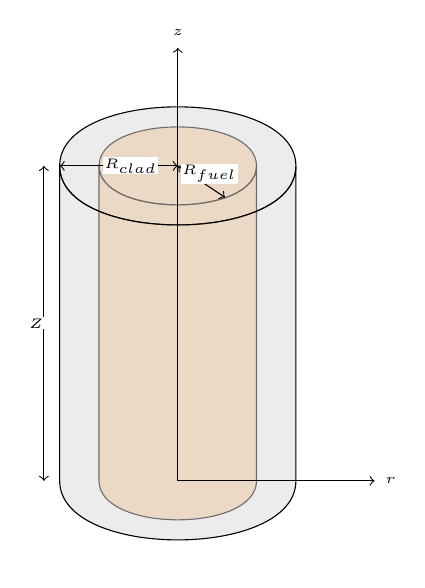
\begin{tikzpicture}

    \tikzstyle{ann} = [fill=white, font=\tiny, inner sep=.5pt]

    % Fuel
    \draw[fill=orange!60, fill opacity=0.5] (0.5,0) to
        [controls=+(90:0.66) and +(90:0.66)] (2.5,0);

    \draw[fill=orange!60, fill opacity=0.5] (0.5,0) .. controls +(-90:0.66)
    and +(-90:0.66) .. (2.5,0);

    \draw[fill=orange!60, fill opacity=0.5] (0.5,0) .. controls +(-90:0.66)
    and +(-90:0.66) .. (2.5,0)
        -- (2.5,-4) .. controls +(-90:0.66) and +(-90:0.66) .. (0.5,-4) -- (0.5,0);


    % Clad
    \draw[fill=lightgray!60, fill opacity=0.5] (0,0) to
        [controls=+(90:1.0) and +(90:1.0)] (3,0);

    \draw[fill=lightgray!60, fill opacity=0.5] (0,0) .. controls +(-90:1.0)
    and +(-90:1.0) .. (3,0);

    \draw[fill=lightgray!60, fill opacity=0.5] (0,0) .. controls +(-90:1.0)
    and +(-90:1.0) .. (3,0)
        -- (3,-4) .. controls +(-90:1.0) and +(-90:1.0) .. (0,-4) -- (0,0);

    % Rfuel and Rclad
    \draw[arrows=<->,line width=.4pt](1.5,0)--(2.1,-.4);
    \draw[arrows=<->,line width=.4pt](1.5,0)--(0,0);
    \node[ann] at (0.9,0) {$R_{clad}$};
    \node[ann] at (1.9,-0.1) {$R_{fuel}$};

    \draw[arrows=<->,line width=.4pt](-0.2,0)--(-0.2,-4);
    \node[ann] at (-0.3,-2) {$Z$};

    % z- and r- axes
    \draw[arrows=->,line width=.4pt](1.5,-4)--(1.5,1.5);
    \draw[arrows=->,line width=.4pt](1.5,-4)--(4.0,-4.0);
    \node[ann] at (1.5,1.7) {$z$};
    \node[ann] at (4.2,-4) {$r$};

    %\node[ann] at (3.5,0.5) {$\Phi=0\mbox{ at }z=Z$};
    %\node[ann] at (3.5,-4.5) {$\Phi=0\mbox{ at }z=0$};

    %\node[ann] at (5.5,-1.3) {$-k_{clad}\nabla T^{clad}
    %                         =h_{conv}(T^{clad}-T_{m})
    %                         \mbox{ at }r=R_{clad}$};
    %\node[ann] at (4.3,-2.8) {$-k_{fuel}\nabla T^{fuel}
    %                           =-k_{clad}\nabla T^{clad}
    %                           =h_{gap}(T^{fuel}-T^{clad})
    %                           \mbox{ at }r=R_{fuel}$};

    %\node[ann] at (3.5,-4.7) {$H=0\mbox{ at }z=0$};

\end{tikzpicture}

